\section{Keep Talking and Nobody Explodes}

\begin{figure}
    \centering
    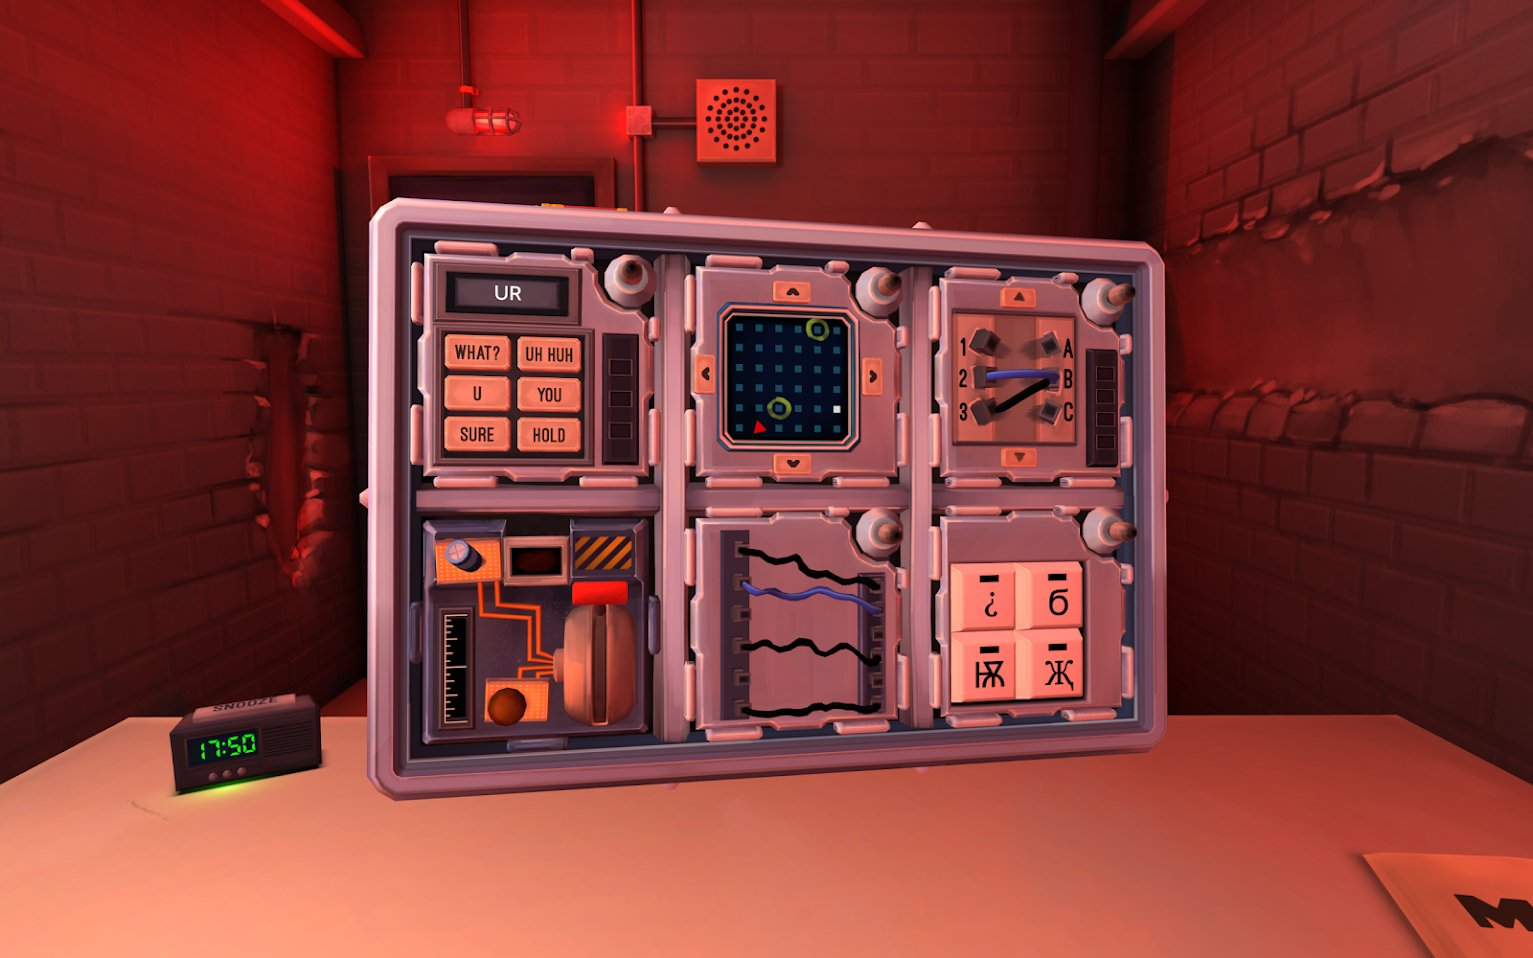
\includegraphics[width=0.5\linewidth]{assets/competitive-apps/keep-talking.jpg}
    \caption{Screenshot hry Keep Talking and Nobody Explodes~\cite{steelcrategamesinc_keep_talking}}
    \label{fig:keep-talking}
\end{figure}

Ve hře \emph{Keep Talking and Nobody Explodes} závisí všechno na správné
kooperaci a~komunikaci.
Tato velmi oceňovaná hra existuje ve verzi pro desktop, konzole,
virtuální realitu i~mobily.~\cite{steelcrategamesinc_keep_talking}

Hra má předpřipravená herní kola s~daným typem bomby.
Bomba je koncipována jako kufřík s~několika moduly a~časomírou,
která se nebezpečně rychle odpočítává.
Jeden hráč vidí bombu.
Další hráč, případně skupina hráčů, mají k~dispozici manuál s~instrukcemi.
Manuál mohou prohlížet jak v~elektronické, tak i~v~papírové podobě.
Manuál je totiž pro všechny hry shodný.

Veškerá komunikace probíhá pouze slovně.
Hráč s~bombou tak nahlásí hráči s~manuálem například to,
že vidí červené tlačítko s~textem \uv{defuse}.
Druhý hráč pak v~manuálu vyhledá daný modul tlačítka, řídí se instrukcemi
a~podstatné informace k~zneškodnění předá prvnímu hráči.

Cíl každého kola je zneškodnění bomby.
Důraz je také kladen na čas zneškodnění a~počet udělaných chyb.
Po skončení kola může hráč porovnat svůj výsledek s~ostatními hráči v~žebříčku.

\subsection*{Klady}

\begin{itemize}
    \item UI je laděné jako pohled na stůl, na kterém je bomba a~časomíra,
    což~dodává hře atmostféru a~vtáhne hráče do děje.
    \item Světla v~místnosti blikají, případně se náhodně vypínají a~zapínají.
    To~přidává na efektu zejména v~situacích,
    kdy zbývá už jen pár sekund a~bomba není dobře vidět.
    \item Přestože je grafika jednodušší, samotná bomba je velmi přehledná.
    \item Manuál je stejný pro všechna herní kola. Lze jej tedy i~vytisknout.
\end{itemize}

\subsection*{Zápory}

\begin{itemize}
    \item U~složitějších modulů je manuál občas hůře pochopitelný.
\end{itemize}
